\bottomheading{$ZZ$ production, processes 81--84, 90}

The $Z$'s can either both decay leptonically ({\tt nproc=81}), one can
decay leptonically while the other decays into neutrinos ({\tt
nproc=82}) or bottom quarks ({\tt nproc=83}), or one decays into
neutrinos and the other into a bottom quark pair ({\tt nproc=84}).  In
process {\tt 83} the mass of the $b$-quark is neglected. Note that, in
processes {\tt 83}--{\tt 84}, the NLO corrections do not include
radiation from the bottom quarks that are produced by the $Z$ decay.
In process {\tt 90} the two $Z$ bosons decay to identical charged
leptons, and interference effects between the decay products of the
two $Z$ bosons are included.  In all cases these processes also
include the contribution from a virtual photon.

When {\tt removebr} is true in process {\tt 81}, neither of the $Z$
bosons decays.

This process has been treated in several papers, 
\cite{Campbell:1999ah,Campbell:2011bn,Boughezal:2016wmq,Campbell:2022gdq}.
Processes {\tt 81} and {\tt 82} can be calculated at NNLO.
The NNLO calculation includes contributions from the process $gg \to ZZ$ 
that proceeds through quark loops. The calculation of loops
containing the third quark generation includes the effect of both the
top and the bottom quark mass ($m_t,m_b \neq 0$), while the first two
generations are considered massless. For numerical stability, a small
cut on the transverse momentum of the $Z$ bosons is applied:
$p_T(Z)>0.1$~GeV.  This typically removes less than $0.1$\% of the
total cross section. The values of these cutoffs can be changed by
editing {\tt src/ZZ/getggZZamps.f} and recompiling.

\bottomheading{Anomalous $WWZ$}

\label{sec:anomalous}
It is possible to specify anomalous trilinear
couplings for the $W^+W^-Z$ and $W^+W^-\gamma$ vertices that are
relevant for $WW$ and $WZ$ production. To run in this mode, one must
set {\tt zerowidth} equal to {\tt .true.}  and modify the appropriate
lines for the couplings in {\tt input.ini} (see below). Note that, at
present, the effect of anomalous couplings is not included in the
gluon-gluon initiated contributions to the $WW$ process.

The anomalous couplings appear in the Lagrangian,
${\cal L} = {\cal L}_{SM} + {\cal L}_{anom}$ as follows
(where ${\cal L}_{SM}$ represents the usual Standard Model Lagrangian and
${\cal L}_{anom}$ is taken from Ref.~\cite{Dixon:1999di}):
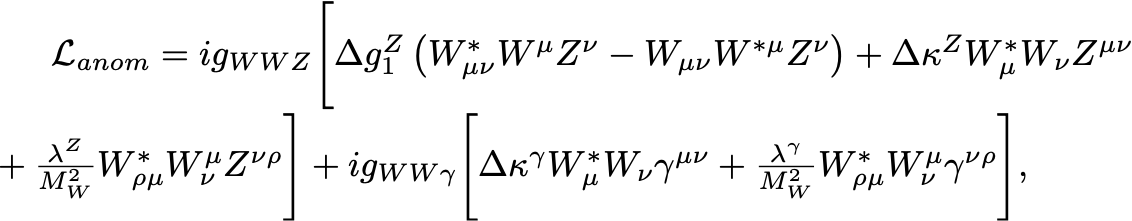
\includegraphics[width=\textwidth]{./sections/gobbets/Lagrangian.png}
%\begin{eqnarray}
%{\cal L}_{anom} & = & i g_{WWZ} \Biggl[
% \Delta g_1^Z \left( W^*_{\mu\nu}W^\mu Z^\nu - W_{\mu\nu}W^{*\mu} Z^\nu \right)
%+\Delta\kappa^Z W^*_\mu W_\nu Z^{\mu\nu} \nonumber \\
% & &+
% \frac{\lambda^Z}{M_W^2} W^*_{\rho\mu} W^\mu_\nu Z^{\nu\rho} \Biggr]
%+i g_{WW\gamma} \Biggl[ 
% \Delta\kappa^\gamma W^*_\mu W_\nu \gamma^{\mu\nu}
%+\frac{\lambda^\gamma}{M_W^2} W^*_{\rho\mu} W^\mu_\nu\gamma^{\nu\rho}
% \Biggr], \nonumber
%\end{eqnarray}

where $X_{\mu\nu} \equiv \partial_\mu X_{\nu} - \partial_\nu X_{\mu}$
and the overall coupling factors are $g_{WW\gamma}=-e$,
$g_{WWZ}=-e\cot\theta_w$.
This is the most general Lagrangian that conserves $C$ and $P$
separately and electromagnetic gauge invariance requires that there
is no equivalent of the $\Delta g_1^Z$ term for the photon coupling.

In order to avoid a violation of unitarity, these couplings are often
included only after suppression by dipole form factors,

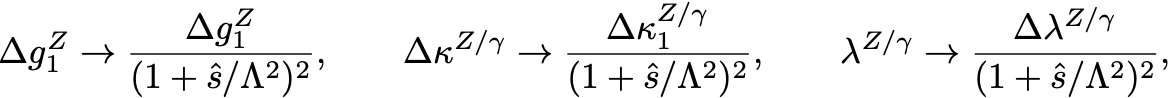
\includegraphics[width=0.9\textwidth]{./sections/gobbets/Dipole.png}

%\begin{equation}
%\Delta g_1^Z \rightarrow \frac{\Delta g_1^Z}{(1+\hat{s}/\Lambda^2)^2}, \qquad
%\Delta \kappa^{Z/\gamma} \rightarrow \frac{\Delta \kappa_1^{Z/\gamma}}{(1+\hat{s}/\Lambda^2)^2}, \qquad
%\lambda^{Z/\gamma} \rightarrow \frac{\Delta \lambda^{Z/\gamma}}{(1+\hat{s}/\Lambda^2)^2},
%\end{equation}
where $\hat{s}$ is the vector boson pair invariant mass and $\Lambda$
is an additional parameter giving the scale of new physics, which should
be in the TeV range.
These form factors should be produced by the new physics associated
with the anomalous couplings and this choice is somewhat
arbitrary. The use of the form factors can be disabled as described
below.  The file {\tt input.ini} contains the values of the $6$
parameters which specify the anomalous couplings.  If the input file
contains a negative value for the form-factor scale then the
suppression factors described above are not applied.

